%%%% Small single column format
\documentclass[anonymous=false, %
               format=acmsmall, %
               review=true, %
               screen=true, %
               nonacm=true]{acmart} 


\usepackage[ruled]{algorithm2e} 
%\usepackage{parskip}
\usepackage{backnaur}
% \usepackage{jlcode}  
\usepackage{todonotes}
\usepackage{alphabeta}
% \usepackage{textalpha}
\usepackage{tikz}
\usepackage{bookmark}
\usetikzlibrary{bayesnet}


\usepackage{graphicx}
\usepackage{subcaption}
\usepackage[utf8]{inputenc}
% \usepackage{unicode-math}
\usepackage{textgreek}
\usepackage{minted} 


\urlstyle{tt}
\citestyle{acmauthoryear}
 
\newmintinline[jl]{julia}{}
\begin{document}

\title{Soss}
%  \titlenote{This is a titlenote}
%  \subtitle{This is a subtitle}
%  \subtitlenote{Subtitle note}

\author{Chad Scherrer}
\orcid{0000-0002-1490-0304}
\affiliation{%
  \institution{RelationalAI}
  % \department{Department of Brain and Cognitive Sciences}
  %\streetaddress{43 Vassar St}
  %\city{Cambridge}
  %\state{MA}
  %\postcode{02139}
  %\country{USA}
}
\email{chad.scherrer@gmail.com}

\author{Taine Zhao}
%\orcid{1234-5678-9012-3456}
\affiliation{%
  \institution{University of Tsukuba}
  \department{Department of Computer Science}
  %\streetaddress{625 Mt Auburn St #3}
  %\city{Cambridge}
  %\state{MA}
  %\postcode{02138}
  %\country{USA}
}
% \email{apfeffer@cra.com}
%\renewcommand\shortauthors{Mage, M. et al}

\begin{abstract}
We present Soss, a declarative probabilistic programming language embedded in the Julia language. Soss represents statistical models in terms of abstract syntax trees, and uses staged compilation for on-demand generation of ``inference primitives'' (random sampling, log-density, etc) without requiring casual users to worry about such details.

The approach taken by Soss makes it easy to extend to take advantage of other packages in the rapidly-growing Julia ecosystem. At the time of this writing, Soss users can choose from several inference back-ends and connect easily with larger systems SymPy and Gen.
\end{abstract}

\maketitle

\section{Introduction}

There are many approaches to building a Probabilistic Programming Language (``PPL''). Soss is distinct from most in a number of ways...







\section{Model syntax}

\begin{figure}[H]
    \centering
    
    \begin{subfigure}[b]{0.4\textwidth}
        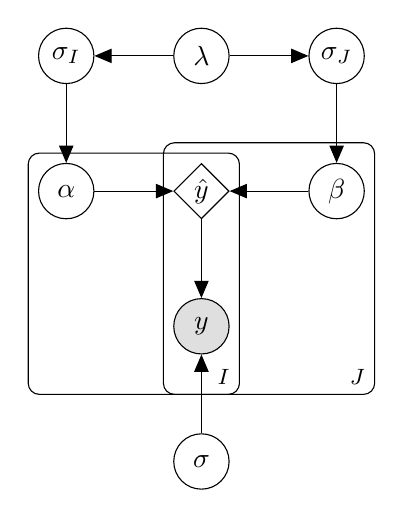
\begin{tikzpicture}

            \node[obs] (y) {$y$};
            \node[det, above=of y] (yhat) {$\hat{y}$};
            \node[latent, left=of yhat] (alpha) {$\alpha$};
            \node[latent, above=of yhat] (lambda) {$\lambda$};
            \node[latent, right=of yhat] (beta) {$\beta$};
            \node[latent, left=of lambda] (sigi) {$\sigma_I$};
            \node[latent, right=of lambda] (sigj) {$\sigma_J$};
            \node[latent, below=of y] (sigma) {$\sigma$};
            
            \edge {sigi} {alpha};
            \edge {sigj} {beta};
            \edge {sigma, yhat} {y};
            \edge {lambda} {sigi};
            \edge {lambda} {sigj};
            \edge {alpha,beta} {yhat};
        
            \plate {I} {(y)(yhat)(alpha)} {$I$};
            \plate {J} {(y)(yhat)(beta)(I.north east)} {$J$};
          
        \end{tikzpicture}
        \caption{}
    \end{subfigure}
    \hspace{0.1in}
    \begin{subfigure}[b]{0.4\textwidth}

    \begin{minted}{julia}
m = @model I,J begin
    λ ~ HalfCauchy()
    σI ~ HalfNormal(λ)
    σJ ~ HalfNormal(λ)
    
    α ~ Normal(0, σI) |> iid(I)
    β ~ Normal(0, σJ) |> iid(J)
    yhat = α .+ β'

    σ ~ HalfNormal()
    y ~ For(I,J) do i,j 
            Normal(yhat[i,j], σ)
        end
    end
    \end{minted} 
    \caption{}
    \end{subfigure}

    \caption{A plate diagram (a) and Soss encoding (b) for a two-way analysis of variance model. Note the specification that $y$ will later be observed is not part of the model, but is instead given at inference time.}
    \label{fig:model}
\end{figure}

Figure~\ref{fig:model} shows a plate diagram and Soss implementation of a simplified two-way ANOVA model. The model $m$ has \emph{arguments} $I$ and $J$. Each line of a model is either a \emph{sample statement} (\jl#v ~ rhs#) or an \emph{assign statement} (\jl#v = rhs#). In either case, \jl#v# must be a valid Julia variable name, and \jl#rhs# must be a valid Julia expression. For a sample statement, \jl#rhs# should also be ``distribution-like'', supporting \jl#logpdf# and/or \jl#rand# methods (depending on the inference algorithm to be used).

\section{Inference Primitives}

A given inference algorithm can be expressed in terms of a collection of functions on a model. For example, we may need to evaluate the log-density or its gradient, map continuous variables into $\mathbb{R}^n$, or draw random samples. In Soss, these \emph{inference primitives} are 


\begin{figure}
    
    \begin{minted}{julia}
        julia> truth = rand(m(I=2,J=3)); pairs(truth)
        pairs(::NamedTuple) with 10 entries:
          :I    => 2
          :J    => 3
          :yhat => [0.0996722 0.720247 -0.706772; 0.100505 0.72108 -0.705939]
          :σ    => 0.297288
          :λ    => 0.523386
          :σJ   => 0.312794
          :σI   => 0.0054669
          :β    => [0.0973136, 0.717889, -0.70913]
          :α    => [0.00235854, 0.00319107]
          :y    => [0.386041 0.564963 -0.72177; 0.236898 0.842491 -0.912154]
    \end{minted}
    
\end{figure}

\section{Model Transformations}


\subsection{Conditional Predictive models}




\subsection{Causal Interventions (``Do'' operator)}

\subsection{Markov Blankets}


\begin{minted}{julia}
julia> markovBlanket(m, :α)
    @model (I, σI, β, σ, J) begin
            α ~ Normal(0, σI) |> iid(I)
            yhat = α .+ β'
            y ~ For(I, J) do i, j
                    Normal(yhat[i, j], σ)
                end
        end
\end{minted}


\section{Symbolic Manipulation}

\subsection{Symbolic Log-density}

\subsection{Code Generation}

\section{Implementation}

\begin{minted}{julia}
struct Model{A,B,M} 
    args  :: Vector{Symbol}
    vals  :: NamedTuple
    dists :: NamedTuple
    retn  :: Union{Nothing, Symbol, Expr}
end
\end{minted}


\section{Performance}

\todo[inline]{Let's implement models from \url{https://statisticalrethinkingjulia.github.io/MCMCBenchmarks.jl/latest/benchmarks/} for benchmark comparisons}

\todo[inline]{Can Soss really generate arbitrary code?}

The ability to generate arbitrary  Julia code makes it difficult to measure performance in Soss. When a performance bottleneck is found, developers or users can ask Soss to generate something different. This design places no a priori constraints on performance.

\todo[inline]{Restructure my writing?}

Besides the purely static code generation via regular macros happening in parsing time, Soss heavily uses a mechanism of "zero-cost" runtime code generation originated by Julia's generated functions \cite{bezanson2012julia}, a.k.a staged functions in the original paper and earlier versions of Julia Programming Language.

The generated functions provide the capability of performing code generation during type inference, generating programs computed by the body of function(a.k.a, generator), once and only once for each combination of argument types.

Further, Julia enables type inference and compiler optimizations equivalent to non-runtime ones in runtime for the callsites of generated functions, hence we gain runtime code generation without losing performance.

To take advantage of this, Soss designs a system to encode sufficient information for generating actual codes, into the types, or objects that can be dispatched like types, which allows the use of generated functions here.

Unfortunately, in current stage, there're some implementation restrictions to Julia's generated functions, and generated functions cannot generate arbitrary Julia codes,
where some advanced programming constructions are missing, such as generators and function-related stuffs like closures(including functions with no free variables), multiple dispatch, etc.

To address this, we introduced the works of easing the restrictions of Julia generated functions,
\todo[inline]{cite GG here?}
which allow us to generate closures from generated functions, and make the programs sufficiently powerful.

Programs that can be generated by Soss are turing complete, as all constructs of Lambda Calculus can be generated.

\begin{minted}{julia}
  abstract type LCTerm end
  struct Lam{Arg, Body <: LCTerm} <: LCTerm end
  struct App{Fn<:LCTerm, Arg<:LCTerm} <: LCTerm end
  struct Var{N} <: LCTerm end
  
  cg(::Type{Lam{Arg, Term}}) where {Arg, Term} = 
    :($Arg -> $(cg(Term)))
  cg(::Type{App{Fn, Arg}}) where {Fn, Arg} = 
    :($(cg(Fn))($(cg(Arg))))
  cg(::Type{Var{N}}) where N = N

  function tolc(expr)
    @match expr begin
      :($f($arg)) => App{tolc(f), tolc(arg)}
      :($x => $y) => Lam{x, tolc(y)}
      a::Symbol => Var{a}
    end
  end
  
  @gg function lc(::Type{Term}) where Term <: LCTerm
      cg(Term)
  end
  
  macro lc(term)
    lc(tolc(term))
  end
  
  x = Core.Box()
  y = Core.Box()
  z = Core.Box()
  f(x) = (x, z)
  @assert (@lc x => x)(x) === (@lc y => y)(x)
  @assert (@lc f => x => f(x))(f)(y) === (y, z)
  \end{minted} 



\section{Extending Soss}

\section{Related Work}

The idea of code generation and symbolic simplification in an embedded PPL goes back to \emph{Passage} \cite{Scherrer2012}. 

\emph{Hakaru} \cite{narayanan2016probabilistic} takes a more ambitious symbolic approach in a stand-alone PPL, allowing a wider variety of program transformations. 

Soss began with a goal of representing models with continuous, fixed-dimensionality parameter spaces, inspired by \emph{Stan} \cite{stan:2017}.

\emph{Gen} \cite{Cusumano-Towner:2019} was developed independently from Soss, but takes a similar approach (and distinct from most PPLs) in its representation of a model as a function from its arguments to a "trace" (to use Gen's terminology). In both Soss and Gen's static DSL, this trace is a mapping from variable names to values. The similarity of these systems makes interoperability relatively straightforward, as demonstrated in \emph{SossGen} (\url{https://github.com/cscherrer/SossGen.jl}).

\emph{Turing} \cite{ge2018t}

\begin{acks}
We would like to acknowledge...
\end{acks}

\bibliographystyle{acm-reference-format}
\bibliography{ref}

\appendix

\section{Model Syntax}

\begin{figure}[!t]
  \centering
  %\fbox{\rule[-.5cm]{0cm}{\linedwid} \rule[-.5cm]{4cm}{0cm}}
  % using the backnaur package
\begin{bnf*}
  \bnfprod{model}{\bnfts{@model} \bnfsp \bnfpn{args} \bnfsp \bnfts{begin} \bnfsp \bnfpn{statements} \bnfsp \bnfts{end}}\\
  \bnfprod{args}{\bnfes \bnfor \bnfpn{Symbol} \bnfor \bnfpn{Symbol} \bnfts{,} \bnfpn{args}} \\
  \bnfprod{statements}{\bnfpn{statement} \bnfor \bnfpn{statement} \bnfsp \bnftd{Julia Line Sep} \bnfsp \bnfpn{statements} \bnfor \bnfpn{statements} \bnfsp \bnfpn{retn}} \\ 
  \bnfprod{statement}{\bnfpn{assign} \bnfor \bnfpn{sample}} \\
  \bnfprod{assign}{\bnfpn{Symbol} \bnfsp \bnfts{=} \bnfsp \bnfpn{Expr}} \\
  \bnfprod{sample}{\bnfpn{Symbol} \bnfsp \bnfts{\textasciitilde}} \bnfsp \bnfpn{Measure} \\
  \bnfprod{retn}{\bnfts{return} \bnfsp \bnfpn{Expr}} \\
  \bnfprod{Symbol}{\bnftd{Julia Symbol}} \\ 
  \bnfprod{Expr}{\bnftd{Julia Expr}} \\
  \bnfprod{Measure}{\bnftd{Probability measure (see text)}}
\end{bnf*}
  \caption{Backus-Naur Form representation for a user-specified model.}
  \label{fig:bnf}
  \Description{Placeholder figure.}
\end{figure}

\section{Symbolic Simplification}
Before simplification:
\[
\begin{aligned}
    \ell = 
       &- 3 \log{\left(2 \right)} 
        - 5 \log{\left(\pi \right)} 
    \\ &- σ^{2} 
        - 4 \log{\left(λ \right)} 
        - 2 \log{\left(λ^{2} + 1 \right)} 
        - \frac{σ_I^{2}}{λ^{2}} 
        - \frac{σ_J^{2}}{λ^{2}}
    \\ &+ \sum_{i=1}^{I} \left(- \log{\left(σ_I \right)} - \frac{\log{\pi }}{2} - \frac{\log{2 }}{2} - \frac{{α}_{i}^{2}}{2 σ_I^{2}}\right) 
    \\ &+ \sum_{j=1}^{J} \left(- \log{\left(σ_J \right)} - \frac{\log{\pi }}{2} - \frac{\log{2 }}{2} - \frac{{β}_{j}^{2}}{2 σ_J^{2}}\right) 
    \\ &+ \sum_{\substack{1 \leq i \leq I \\ 1 \leq j \leq J}} \left(- \log{\left(σ \right)} - \frac{\log{\pi }}{2} - \frac{\log{2 }}{2} - \frac{\left({y}_{ij} - {\hat{y}}_{ij}\right)^{2}}{2 σ^{2}}\right) 
\end{aligned}
\]

After simplification:
\[
    \begin{aligned}
    \ell =
    &- 7.8 - 0.92 I - 0.92 J - 0.92 I J 
    \\ &- 4 \log{λ } - 2 \log{\left(λ^{2} + 1 \right)} 
        - σ^{2} 
        - I J \log{σ } 
    \\ &- I \log{σ_I } - J \log{σ_J } - \frac{σ_I^{2}}{λ^{2}}  - \frac{σ_J^{2}}{λ^{2}}
    \\ &- \frac{1}{2 σ_I^{2}} \sum_{i=1}^{I} {α}_{i}^{2}
        - \frac{1}{2 σ_J^{2}} \sum_{j=1}^{J} {β}_{j}^{2}
        - \frac{1}{2 σ^{2}} \sum_{\substack{1 \leq i \leq I\\1 \leq j \leq J}} \left({y}_{ij} - {\hat{y}}_{ij}\right)^{2}
    \end{aligned}
\]


\end{document}
